%%%%%%%%%%%%%%%%%%%%%%%%%%%%%%%%%%%%%%%%%
% Short Sectioned Assignment
% LaTeX Template
% Version 1.0 (5/5/12)
%
% This template has been downloaded from:
% http://www.LaTeXTemplates.com
%
% Original author:
% Frits Wenneker (http://www.howtotex.com)
%
% License:
% CC BY-NC-SA 3.0 (http://creativecommons.org/licenses/by-nc-sa/3.0/)
%
%%%%%%%%%%%%%%%%%%%%%%%%%%%%%%%%%%%%%%%%%

%----------------------------------------------------------------------------------------
%	PACKAGES AND OTHER DOCUMENT CONFIGURATIONS
%----------------------------------------------------------------------------------------

\documentclass[paper=a4, fontsize=12pt]{scrartcl} % A4 paper and 11pt font size

\usepackage[margin=1.0in]{geometry}

\usepackage[T1]{fontenc} % Use 8-bit encoding that has 256 glyphs
\usepackage{fourier} % Use the Adobe Utopia font for the document - comment this line to return to the LaTeX default
\usepackage[english]{babel} % English language/hyphenation
\usepackage{amsmath,amsfonts,amsthm} % Math packages

\usepackage{lipsum} % Used for inserting dummy 'Lorem ipsum' text into the template

\usepackage{sectsty} % Allows customizing section commands
\allsectionsfont{\centering \normalfont\scshape} % Make all sections centered, the default font and small caps

\usepackage{IEEEtrantools}
\usepackage{listings}
\usepackage{caption}
\usepackage{subcaption}
\usepackage{graphicx}

\usepackage{fancyhdr} % Custom headers and footers
\pagestyle{fancyplain} % Makes all pages in the document conform to the custom headers and footers
\fancyhead{} % No page header - if you want one, create it in the same way as the footers below
\fancyfoot[L]{} % Empty left footer
\fancyfoot[C]{} % Empty center footer
\fancyfoot[R]{\thepage} % Page numbering for right footer
\renewcommand{\headrulewidth}{0pt} % Remove header underlines
\renewcommand{\footrulewidth}{0pt} % Remove footer underlines
\setlength{\headheight}{13.6pt} % Customize the height of the header

\numberwithin{equation}{section} % Number equations within sections (i.e. 1.1, 1.2, 2.1, 2.2 instead of 1, 2, 3, 4)
\numberwithin{figure}{section} % Number figures within sections (i.e. 1.1, 1.2, 2.1, 2.2 instead of 1, 2, 3, 4)
\numberwithin{table}{section} % Number tables within sections (i.e. 1.1, 1.2, 2.1, 2.2 instead of 1, 2, 3, 4)

%\setlength\parindent{0pt} % Removes all indentation from paragraphs - comment this line for an assignment with lots of text

%----------------------------------------------------------------------------------------
%	TITLE SECTION
%----------------------------------------------------------------------------------------

\newcommand{\horrule}[1]{\rule{\linewidth}{#1}} % Create horizontal rule command with 1 argument of height

\title{	
\normalfont \normalsize 
\textsc{Department of EE - IIT Madras} \\ [25pt] % Your university, school and/or department name(s)
\horrule{0.5pt} \\[0.4cm] % Thin top horizontal rule
\huge Assignment 3 \\Protograph Thresholds and Code Design % The assignment title
\horrule{2pt} \\[0.5cm] % Thick bottom horizontal rule
}

\author{Surajkumar Harikumar (EE11B075)} % Your name

\date{\normalsize\today} % Today's date or a custom date

\begin{document}

\maketitle % Print the title

%----------------------------------------------------------------------------------------
%	PROBLEM 1
%----------------------------------------------------------------------------------------

\section{Problem Statement}

Given the base parity check matrix of a protograph, find its BEC threshold. Design a protograph with the highest threshold, given the number of variable nodes, check nodes, and total number of edges. 

\section{Threshold Finding}

A protograph is completely specified by its base matrix, which denote the number of connections from a variable node to a check node.  We introduce the notion of an edge type, so that we can write out exact equations for message passing (rather than the averaged ones we had in LDPC codes). We can write a set of vector-density evolution equations for the protograph, based on message-passing decoding.
\\ \\
For simplicity all edges between the same variable node and check node are assumed to be of the same type (as they have the same neighbourhood on both end nodes). So we have one edge type corresponding to each entry in the $H$-matrix, and each edge type has a multiplicity specified by its $H$-matrix entry
\\ \\
The protograph is then copy-permuted, where we copy the base protograph, say $L$-times, and then permute the edges of the same type. The benefit of doing this is that the density evolution equations for the resulting LDPC-code is the same as that of the base protograph. So we have an exact way to track the evolution of messages in the LDPC code. 

\pagebreak
\subsection{Density evolution}

We formulated density evolution equations for protographs as seen in \cite{Lent}. The density evolution equation is  completely specified by the base matrix, and for any $e_{i,j}$-edge type, we need only look at the row and column neighbourhood. The script \textbf{proto\_de\_iter.m} takes in the parity check matrix, $\epsilon$ and number of iterations as input, and returns the edge-erasure probabilities in each iteration. The \textbf{status} variable, tells us if DE converges to zero during the iterations. 

\begin{figure}
\centering
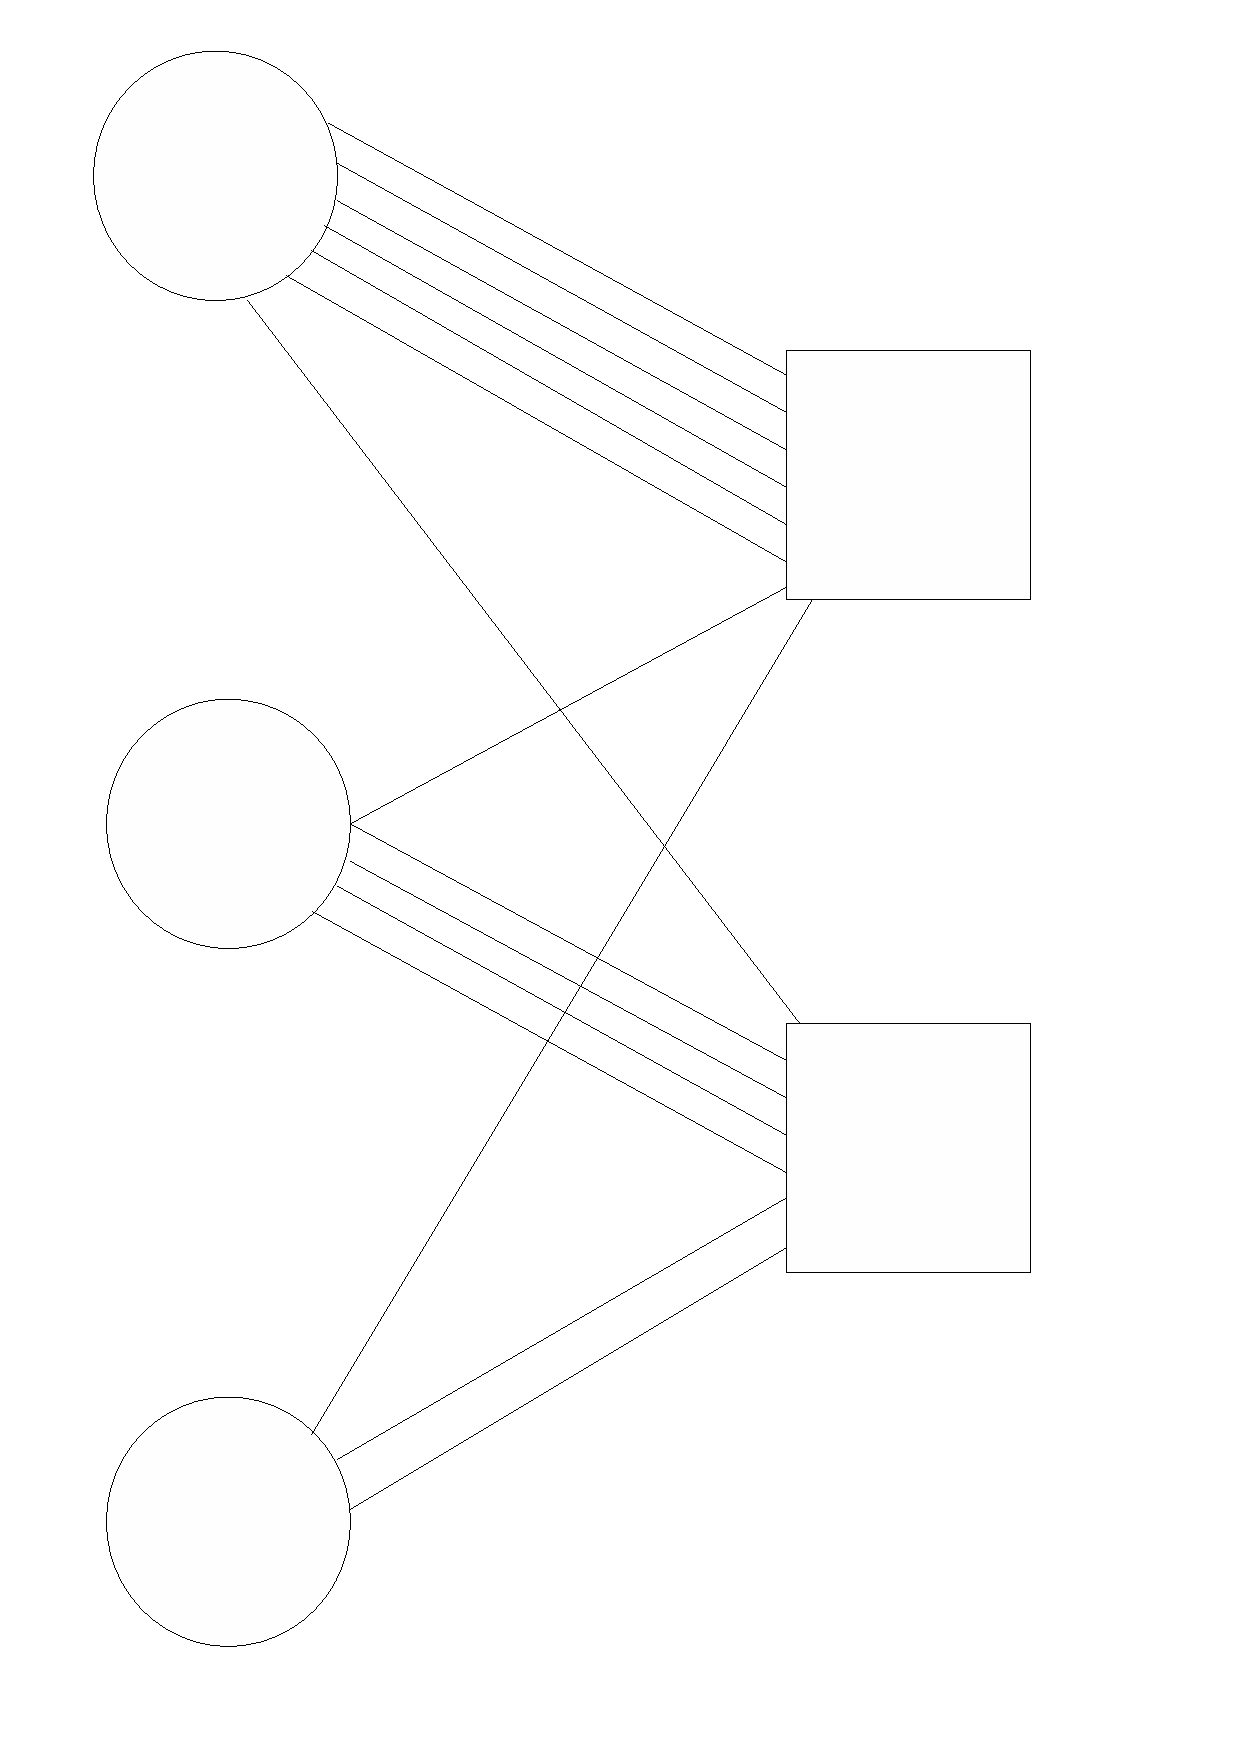
\includegraphics[width=0.3\textwidth]{images/modified-proto}
\caption{Rate $1/3$ protograph with 3 variable nodes, 2 check nodes, and 15 edges. }
\label{proto}
\end{figure}

\subsection{Threshold Finding and Simulation}
For finding the threshold, we simply iterate over values of $\epsilon$ till DE stops converging to zero. We start with low values of $\epsilon$ and keep increasing till DE stops converging to zero say at $\epsilon_1$(status variable holds False). Say the immediate previous value was $\epsilon=\epsilon_0$. We now check at $\epsilon_2 = 0.5(\epsilon_0+\epsilon_1)$. If this converges, the threshold is above $\epsilon_2$, so repeat setting $\epsilon_0=\epsilon_2$. Else, set $\epsilon_1=\epsilon_2$. We keep dividing the interval into 2, and we iterate till we get a 4-digit accurate threshold. The script \textbf{proto\_thresh\_brute.m} implements this.
\\ \\
We used the protograph shown in Figure (\ref{proto}), and ran the threshold finder. The BEC threshold was found to be $\epsilon^* = 0.4594$. Figure (\ref{de}) shows the density evolution run at $\epsilon$ just below the threshold. Each blue-line represents a different edge-type. We see that it converges to zero sharply after about 200 iterations. The script \textbf{sub\_test.m} is used to implement this. 


\begin{figure}[h]
\centering
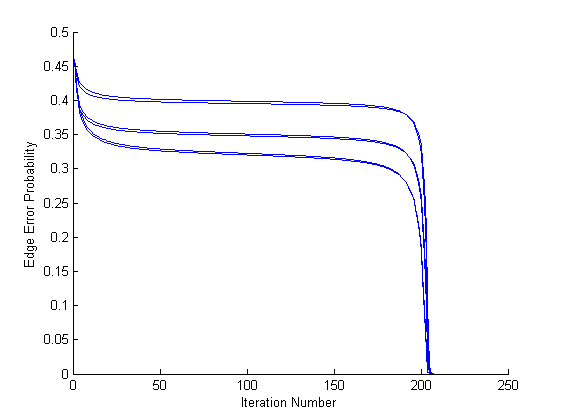
\includegraphics[width=0.8\textwidth]{images/proto-de}
\caption{Density evolution run at $\epsilon = 0.4593$ }
\label{de}
\end{figure}


\pagebreak
\section{Finding the Best protograph}
We need to find the protograph with the highest threshold, given the number of variable nodes N, check nodes M, and total number of edges L. This is equivalent to finding all parity check matrices, such that the sum of all elements in the $H$-matrix equals the number of edge types. This is no easy task, as the search space can be large.
\\ \\
We implemented a brute force search, specific to $N=3,M=1$ in the script \textbf{proto\_best.m}. We scan through all possible H-matrices, find their thresholds and choose the best. Even for $L=10$, there were about $37$ possible protographs. 
\\ \\
We found $\epsilon^*_{best} = 0.2897$, corresponding to $H=\left[5,3,2\right]$. For the rate 2/3 code, we know that $\epsilon* \leq 1 - R = 0.3333$. Our optimization gave $\epsilon^*_{best} = 0.2897$, which is reasonably close to the upper bound. 

For us to extend this to the general case, we can use recursions and loops. However the search space is just too vast for a brute force search to work well. 

\begin{thebibliography}{155}
\bibitem{Lent}
Lentmaier, M. ; Tavares, M.B.S. ; Fettweis, G.P. \textit{"Exact erasure channel density evolution for protograph-based generalized LDPC codes"}, ISIT 2009

\end{thebibliography}

\end{document}

